\documentclass[serif,mathserif, 12pt]{beamer}
\usepackage{etex}
\usepackage{amsmath, amsfonts, epsfig, xspace}
\usepackage{algorithm,algorithmic}
\usepackage{pstricks,pst-node}
\usepackage{multimedia}
\usepackage[normal,tight,center]{subfigure}
\setlength{\subfigcapskip}{-.5em}
\usepackage{beamerthemesplit}
\usetheme{lankton-keynote}
\usepackage{graphicx,color}
% remove caption of figure
\usepackage[labelformat=empty]{caption}

\usepackage[none]{hyphenat} % hyphenation is ugly in slides
\usepackage{parskip}

\usepackage{relsize} % \smaller to change size

\usepackage{tikz}
\usetikzlibrary{calc}

\usetikzlibrary{arrows}

\newcommand{\TikzDraw}[2][]{
  \begin{tikzpicture}[overlay, remember picture, shift={(current page.center)}, #1]
    #2
  \end{tikzpicture}
}

\newcommand{\gridlines}{
  \TikzDraw{
    \draw[help lines,xstep=.2,ystep=.2,red!20] (current page.south west) grid (current page.north east);
    \draw[help lines,xstep=1,ystep=1,red] (current page.south west) grid (current page.north east);
    \foreach \x in {-15,-14,...,15} {
      \node [anchor=north, red] at (\x,0) {\tiny \x};
      \node [anchor=east,red] at (0,\x) {\tiny \x};
    }
  }
}

\newcommand{\DrawOnImg}[3][]
{
  \begin{tikzpicture}
    \node[anchor=south west,inner sep=0] (image) at (0,0){
      #2
    };
    \begin{scope}[x={(image.south east)},y={(image.north west)}]
      \ifthenelse{\equal{#1}{grid}}
                 {\draw[color=blue, style=dashed] (0,0) grid[xstep=.1, ystep=.1] (1.0001,1.0001);}
                 {}
                 #3
    \end{scope}
  \end{tikzpicture}
}

\usetikzlibrary{matrix}

\newcommand{\BOLD}[1]{\mathbf{#1}}
\newcommand{\BOLDG}[1]{\boldsymbol{#1}}
\newcommand{\PDIF}[2]{\frac{\partial #1}{\partial #2}}
\newcommand{\TODO}[1]{\textcolor{red}{#1}}
\newcommand{\TODOB}[1]{\textcolor{blue}{#1}}
\newcommand{\TODOG}[1]{\textcolor{green!50!black}{#1}}
\newcommand{\argmin}{\operatornamewithlimits{arg\min}}
\DeclareMathOperator{\tr}{tr}
\DeclareMathOperator{\cond}{cond}
\DeclareMathOperator{\ST}{s.t.}
\DeclareMathOperator{\diag}{diag}
\DeclareMathOperator{\Div}{div}

\author[Jiong Chen]{Jiong Chen}

\title[\hspace{2em}\insertframenumber/\inserttotalframenumber]{Polyharmonic homogenization, rough polyharmonic splines and sparse super-localization}
\date{October 19, 2017}

% \institute{Zhejiang University}

\begin{document}

\maketitle

\begin{frame}
  \frametitle{Terminology}
  \begin{itemize}
  \item Harmonic
    \begin{equation*}
      \Delta f = 0
    \end{equation*}
  \item Polyharmonic
    \begin{equation*}
      \Delta^m f = 0
    \end{equation*}
  \item Polyharmonic spline
    \begin{equation*}
      \begin{split}
       & f(\BOLD{x}) = \sum_i^N w_i\phi(|\BOLD{x}-\BOLD{c_i}|)+\BOLD{v}^T
      \begin{pmatrix}
        1 \\ \BOLD{x} 
      \end{pmatrix} \\
      &\text{where}\quad \Delta ^m \phi = \delta(x)
      \end{split}
    \end{equation*}
    \item Rough: not smooth
  \end{itemize}
\end{frame}

\begin{frame}
  \frametitle{Homogenization}
  \begin{itemize}
  \item The process of making things uniform or similar.
  \item Less degree of freedoms.
  \end{itemize}
  \TikzDraw {
    \node at (0, -1.6) {
\includegraphics[width=0.5\textwidth]{img/spring}};
  }
\end{frame}

\begin{frame}
  \frametitle{Problem definition}
  \begin{itemize}

  \item Rough harmonic equation
    \begin{equation*}
    \begin{split}
    &\begin{cases}
      &-\Div (a(x)\nabla u(x)) = g(x), \\
      &x\in \Omega; g\in L^2(\Omega), a(x) = \{a_{ij} \in L^\infty(\Omega)\} \\
      &u = 0, x \in \partial\Omega
    \end{cases} \\
    &\lambda_{\min}(a)|\xi|^2 \le \xi^Ta(x)\xi \le \lambda_{\max}(a)|\xi|^2
    \end{split}
    \end{equation*}
    \pause
  \item Homogenization in classical sense
    \begin{equation*}
      \begin{split}
        &a(x) = a(x, \epsilon), \\
        &\epsilon \rightarrow 0, u_\epsilon \rightarrow u_0, -\Div(\TODO{\hat a} \nabla u_0) = g,
      \end{split}
    \end{equation*}
    \pause
  \item Homogenization in numerical sense
    \begin{itemize}
    \item[-] approximate solution space by a finite dimensional space.
    \end{itemize}
  \end{itemize}
\end{frame}

\begin{frame}
  \frametitle{Functional space approximation}
  \TikzDraw {
    \node at (-2, -1) {
      \parbox[h]{0.8\textwidth}{
        \begin{itemize}
          \visible<1-> {
      \item Finite dimensional approximation
        \begin{equation*}
          x(\xi) = \sum_{i=1}^n y_i\phi_i(\xi)
        \end{equation*}
          }
          \visible<3-> {
      \item Distance between func space
        \begin{equation*}
          d(X_n, A) = \sup_{x\in A} \inf_{y_n \in X_n}\|x-y_n\|_X
        \end{equation*}
        \end{itemize}
        }
      }      
    };
    \visible<1> {
      \node at (3.5, -0.5) {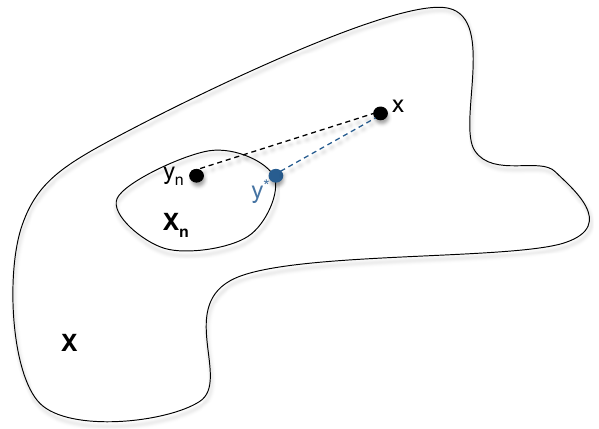
\includegraphics[width=0.5\textwidth]{img/func_distance}};
    }
    \visible<2> {
      \node at (3.5, -0.5) {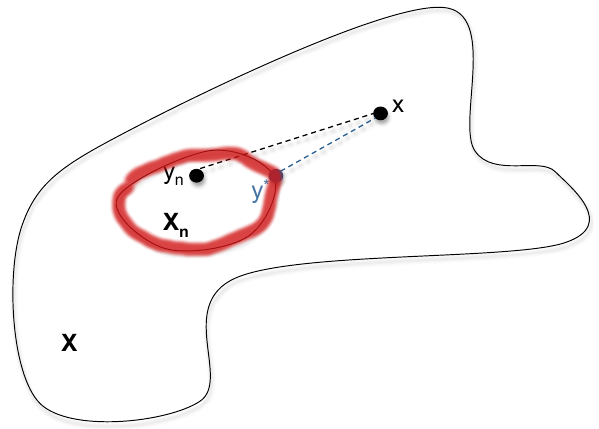
\includegraphics[width=0.5\textwidth]{img/func_distance_highlight}};
    }
    \visible<3> {
      \node at (3.5, -0.5) {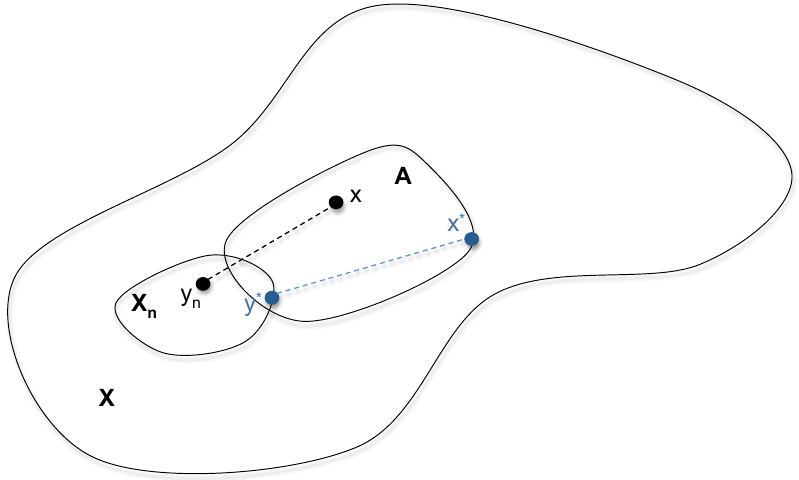
\includegraphics[width=0.5\textwidth]{img/func_space_distance}};
    }
  }
\end{frame}


\begin{frame}
  \frametitle{Pipeline}
  \begin{itemize}
  \item Discretization $(x_i)_{i\in \mathcal{N}}$ with $\mathcal{N}:=\{1, \dots, N\}$.
  \item Identify the nodal interpolation basis $(\phi_i)_{i \in \mathcal{N}}$.
  \item Evaluate the approximation solution space.
    \pause
    \TODO{
    \item Mesh norm
      \begin{equation*}
        H := \sup_{x\in \Omega}\min_{i\in \mathcal{N}} |x-x_i|
      \end{equation*}
    }
  \end{itemize}
\end{frame}

\begin{frame}
  \frametitle{Basis optimization}
  \TikzDraw {
    \node at (-1.8, -0.5) {
    \parbox[h]{0.8\textwidth} {
  \begin{itemize}
  \item Formulation
    \begin{equation*}
      \begin{split}
        &\min_{\phi_i} \int_{\Omega} |\Div(a\nabla \phi_i)|^2 \\
        &\ST \phi_i(x_j) = \delta_{ij}
      \end{split}
    \end{equation*}
    \pause
  \item Accuracy of $u^{in}(x) = \sum_{i=1}^N u(x_i)\phi_i(x)$
    \begin{equation*}
      \begin{split}
      \|u-u^{in}\|_{\mathcal{H}_0^1(\Omega)} \le CH\|g\|_{L^2(\Omega)} \\
      C = C(\lambda_{\min}(a), \lambda_{\max}(a), \Omega)
      \end{split}
    \end{equation*}
  \end{itemize}
  }};
  }
  \TikzDraw {
    \node at (4, -0.5) {\scriptsize{
      \parbox[h]{\textwidth} {
        \begin{equation*}
          \boxed{
            \begin{split}
              &\begin{cases}
                 &-\Div (a(x)\nabla u(x)) = g(x), \\
                 &x\in \Omega; g\in L^2(\Omega), \\
                 &a(x) = \{a_{ij} \in L^\infty(\Omega)\} \\
                 &u = 0, x \in \partial\Omega
               \end{cases} \\
              &\lambda_{\min}(a)|\xi|^2 \le \xi^Ta(x)\xi \le \\
              &\lambda_{\max}(a)|\xi|^2
            \end{split}
            }
        \end{equation*}
        }
      }
    };
  }
\end{frame}

\begin{frame}
  \frametitle{Localization}
  \begin{itemize}
    \visible<1-> {
  \item Localization on subset $\Omega_L \subseteq \Omega$
    \begin{equation*}
      \begin{split}
      &\min \int_{\Omega_L} |\Div (a\nabla \phi_i) |^2 \\
      &\ST \phi_i(x_j) = \delta_{ij} \\
      &~~~~~~~\phi_i = 0 ~\text{on}~ \partial\Omega_L \cup (\Omega \setminus \Omega_L)
      \end{split}
    \end{equation*}
    }
    \visible<2-> {
  \item Accuracy
    \begin{equation*}
      \|u-u^{H, loc}\|_{\mathcal{H}_0^1(\Omega)} \le C\|g\|_{L^2(\Omega)}(H+N\max_{i\in \mathcal{N}}
      \|\phi_i - \phi_i^{loc}\|_{\mathcal{H}^1_0(\Omega)})
    \end{equation*}
    }
  \end{itemize}
  \TikzDraw {
    \node at (4, 1.8) {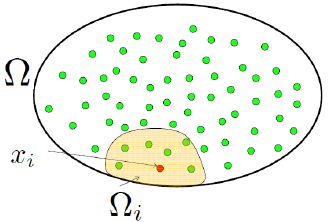
\includegraphics[width=0.3\textwidth]{img/local_domain}};
  }
\end{frame}

\begin{frame}
  \frametitle{Numerical Implementation}
  \begin{itemize}
  \item Discretization $\mathcal{T}_H$ and $\mathcal{T}_h$.
    \begin{figure}
      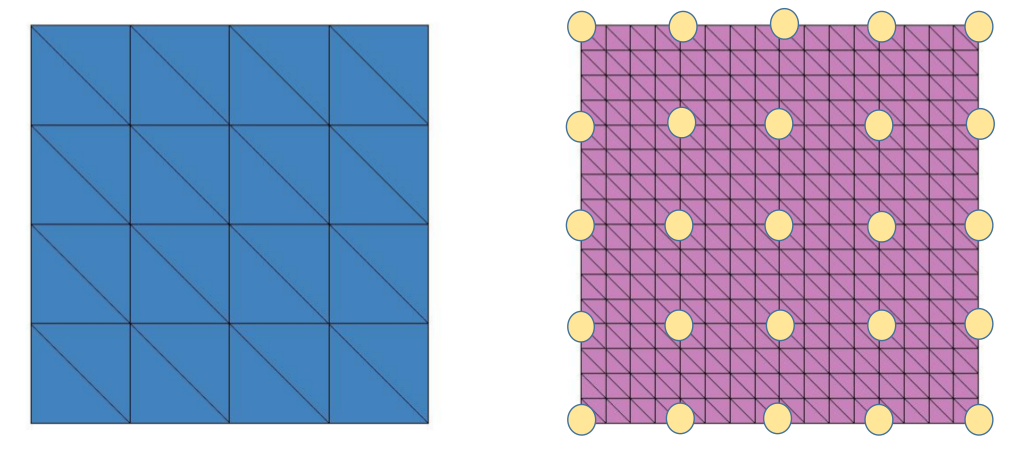
\includegraphics[width=0.4\textwidth]{img/ThandTH}
    \end{figure}
    \pause
  \item $W_h(\Omega)$ set of piecewise linear functions on $\mathcal{T}_h$ with zero Dirichlet boundary
    condition
    \pause
    \visible<3> {\item Discrete optimization
    \begin{equation*}
      \begin{split}
        &\min \int_{\Omega_L} |g_\phi|^2 dx \\
        &\ST \phi \in W_h(\Omega_L), \phi = 0~\text{on}~\partial\Omega_L \cup \Omega\setminus \Omega_L \\
        &~~~~~~\phi(x_j) = \delta_{ij}, j \in \mathcal{N}
      \end{split}
    \end{equation*}
    }
  \end{itemize}
  \TikzDraw {
    \visible<3> {
      \node at (4, -1.4) {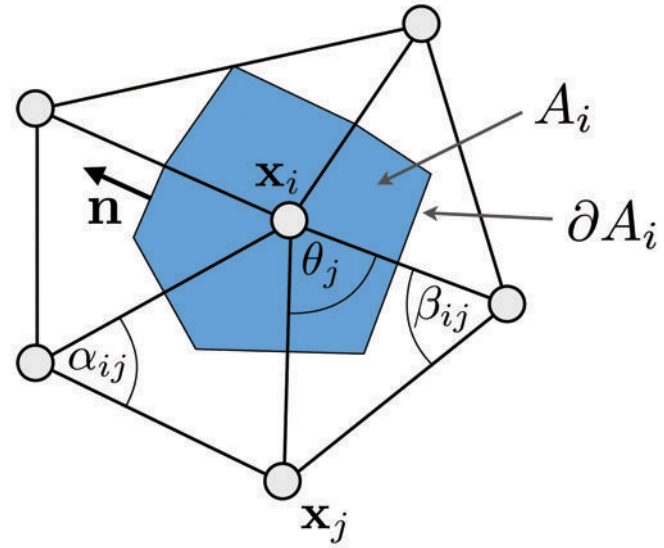
\includegraphics[width=0.3\textwidth]{img/voronoi}};
      }
    \visible<4> {
      \node at (0, -2) {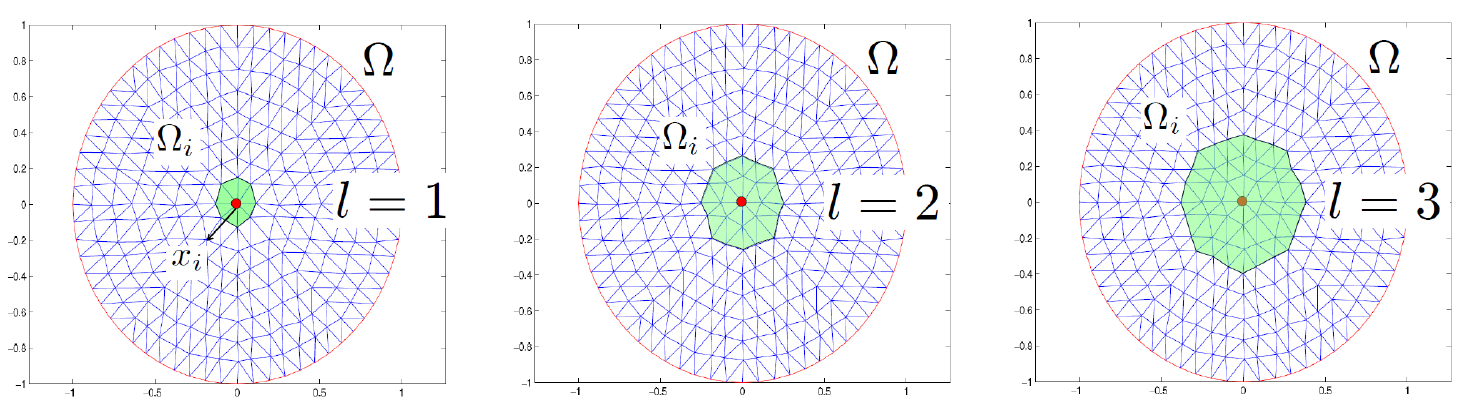
\includegraphics[width=0.8\textwidth]{img/layers}};
    }
  }
\end{frame}

\begin{frame}
  \frametitle{Results}
  \begin{itemize}
  \item Coefficients $a(x)$
    \begin{figure}
      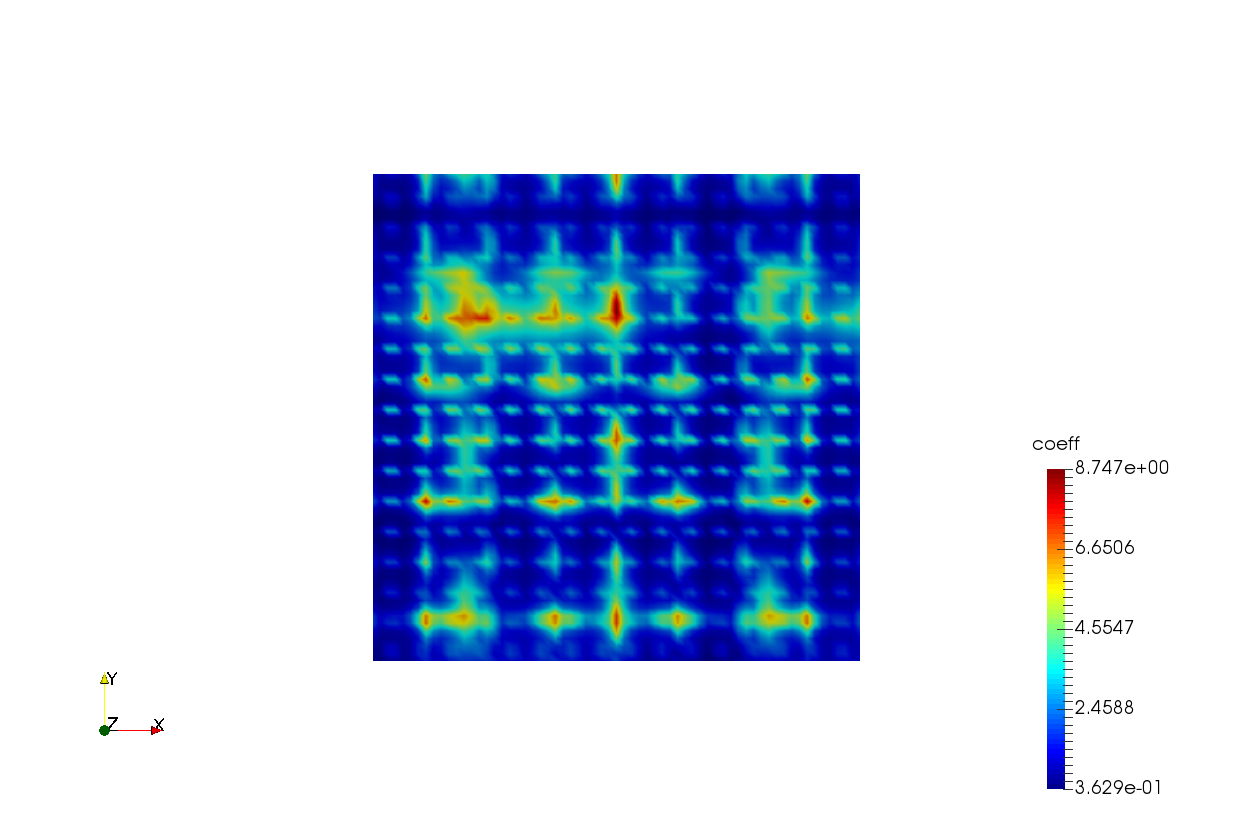
\includegraphics[width=0.8\textwidth]{img/fielda}
    \end{figure}
  \end{itemize}
\end{frame}

\begin{frame}
  \frametitle{Results}
  \begin{itemize}
  \item Optimized basis
    \begin{figure}
      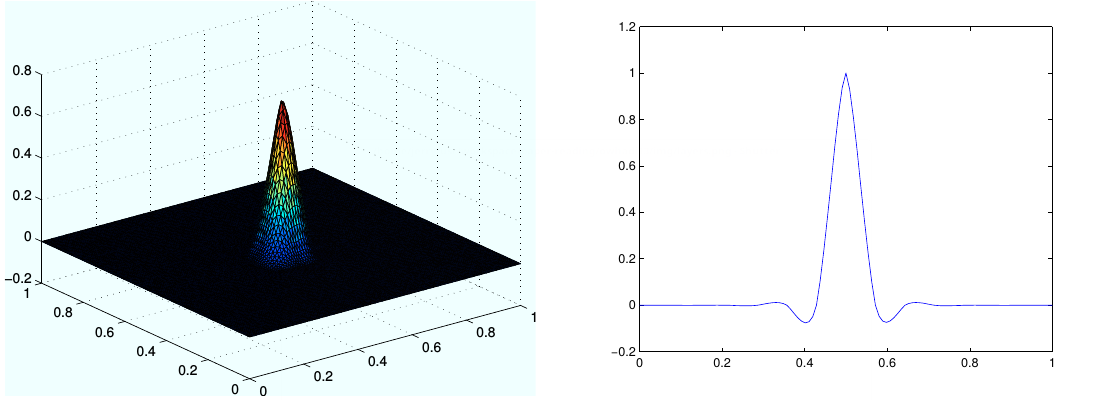
\includegraphics[width=0.8\textwidth]{img/optimized_basis}
    \end{figure}
  \end{itemize}
\end{frame}

\begin{frame}
  \frametitle{Results}
  \begin{itemize}
  \item My results
    \begin{figure}
      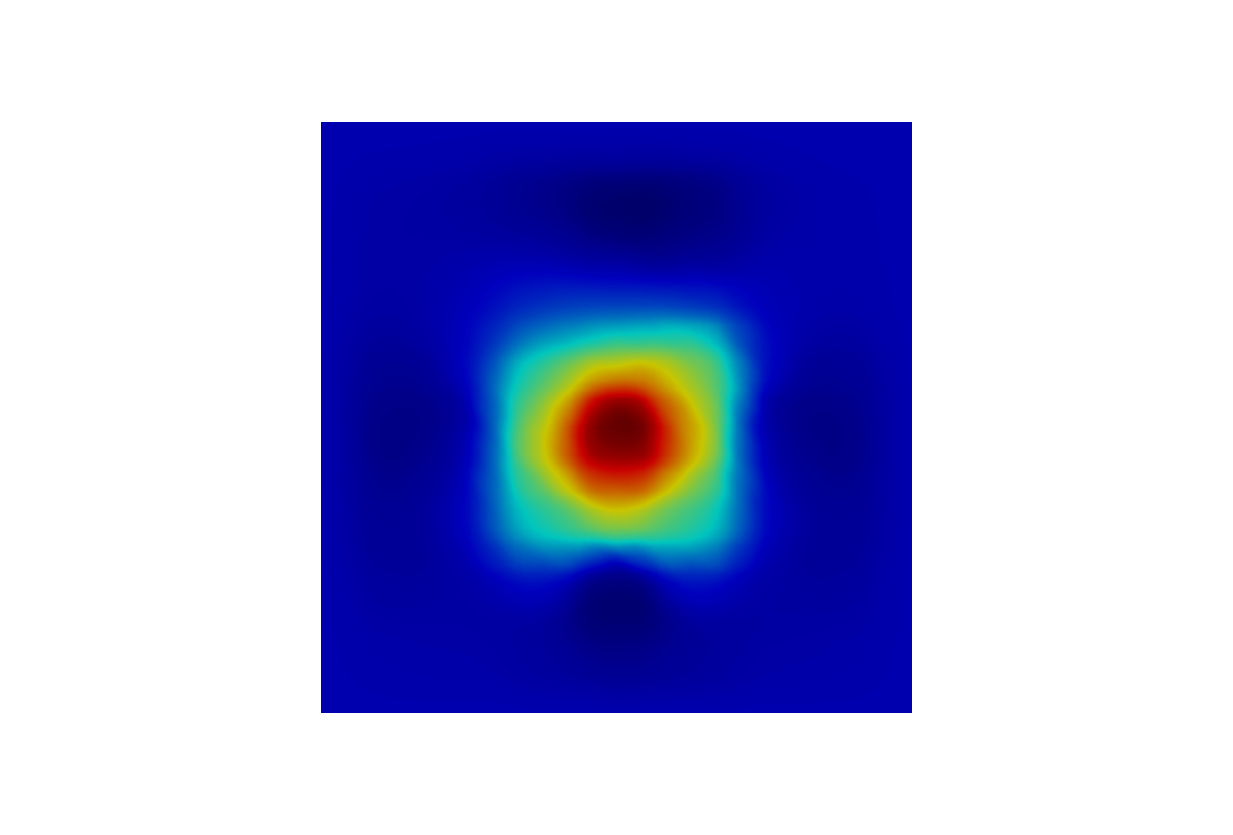
\includegraphics[width=0.8\textwidth]{img/my_optimal_basis}
    \end{figure}
  \end{itemize}
\end{frame}

\begin{frame}
  \frametitle{Results}
  \begin{itemize}
  \item Optimized harmonic basis
    \begin{figure}
      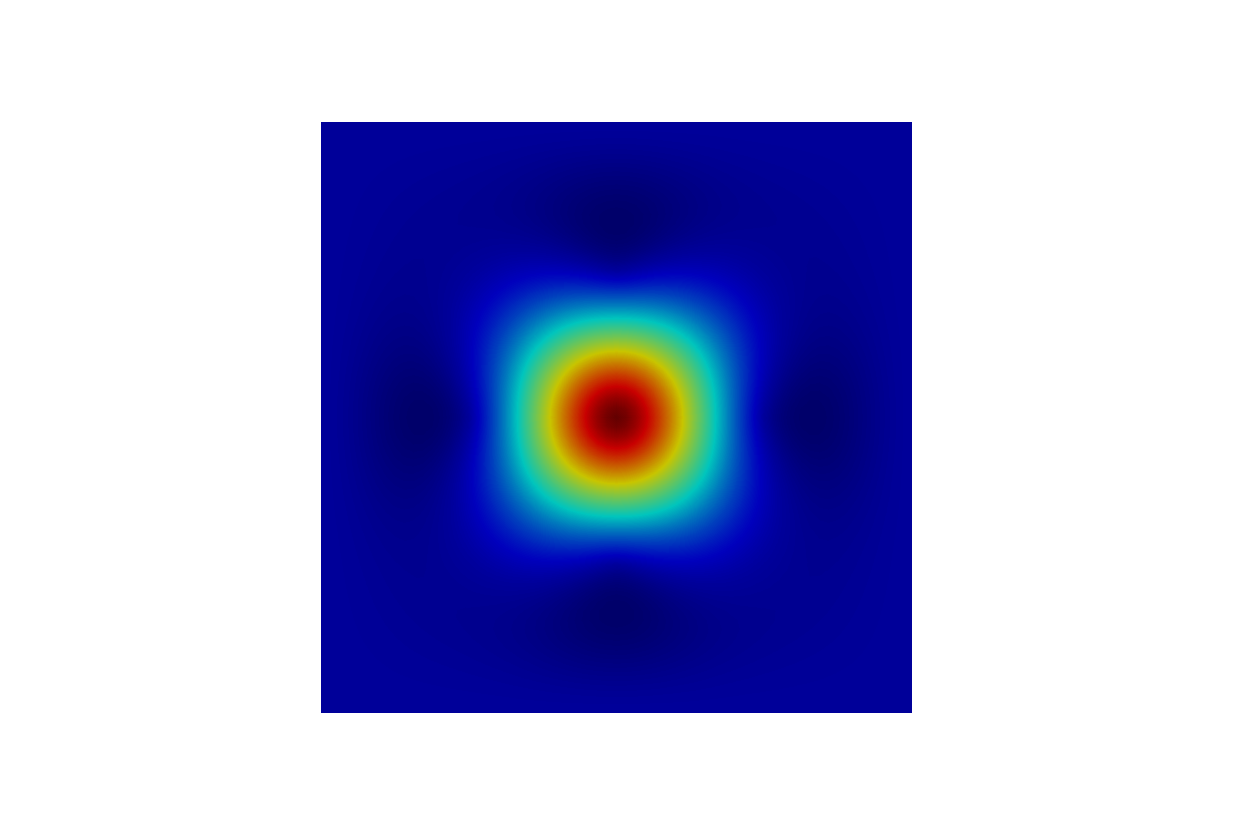
\includegraphics[width=0.8\textwidth]{img/my_harmonic_basis}
    \end{figure}
  \end{itemize}
\end{frame}

\begin{frame}
  \frametitle{Results}
  \begin{itemize}
  \item Accuracy of the interpolation basis
    \begin{figure}
      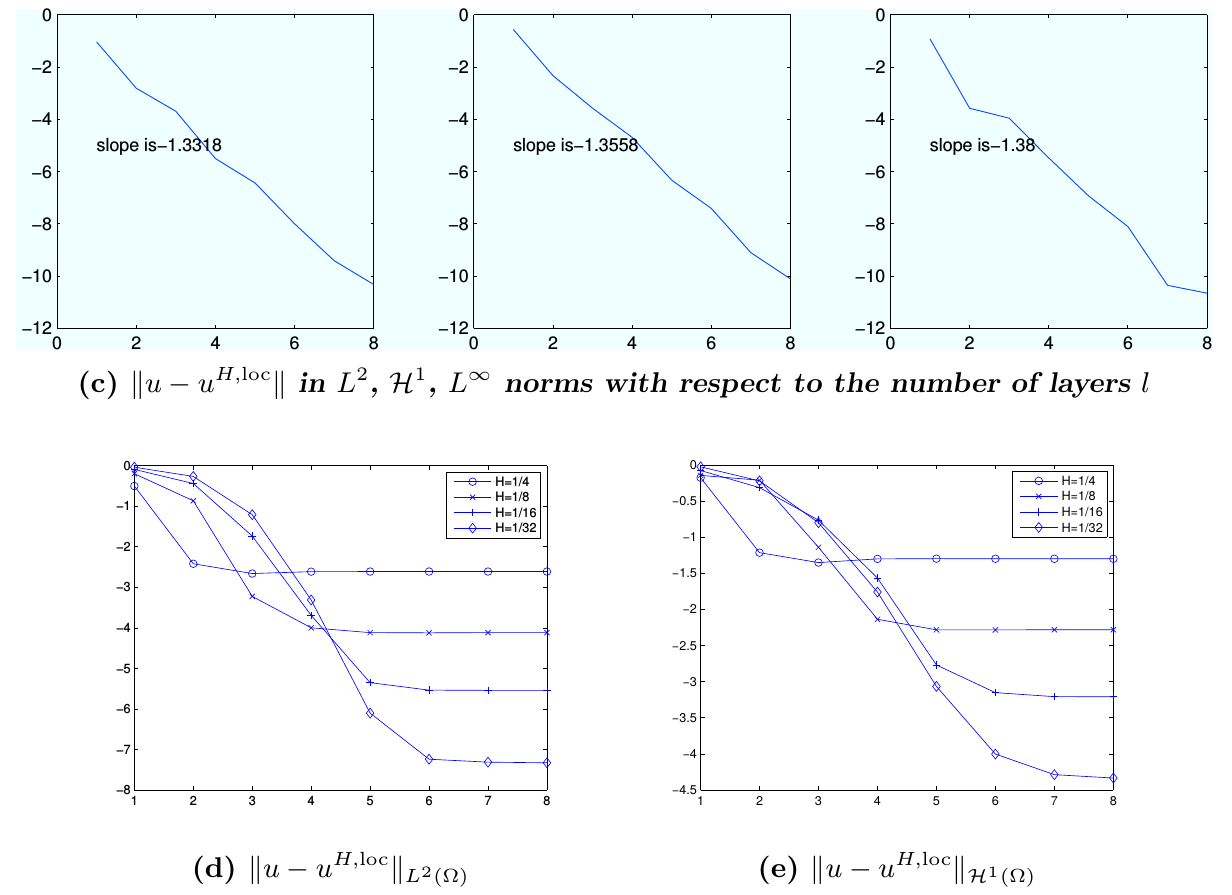
\includegraphics[width=0.8\textwidth]{img/in_basis_accuracy}
    \end{figure}
  \end{itemize}
\end{frame}

\begin{frame} 
  \TikzDraw {
    \node at (0, 0.5) {\Huge{Thanks!}};
  }
  %\gridlines
\end{frame}

\end{document}
